\documentclass[20pt]{beamer}
\usepackage[utf8]{inputenc}
\usepackage[T1]{fontenc}
\usepackage{lmodern}
\usepackage{graphics}
\usepackage{booktabs}
\usepackage{wasysym}
\usepackage{colortbl}
\usepackage{multirow}

\graphicspath{{../../graphs}}
\usetheme{Jacquenetta}

\newcommand{\sigyes}{\checked}
\newcommand{\signo}{$\times$}

\begin{document}
	\author{Dimitris Tsirmpas}
	\title{When Silver Isn't Gold: Quantifying and Auditing Group-Based Disagreement in Human and LLM Annotation}
	%\subtitle{}
	%\logo{}
	%\institute{}
	%\date{}
	%\subject{}
	%\setbeamercovered{transparent}
	%\setbeamertemplate{navigation symbols}{}
	\begin{frame}[plain]
		\maketitle
	\end{frame}
	
	\section{Intro and Motivation}
	
	\begin{frame}{Terminology}
		\begin{enumerate}
			\item \textbf{Disagreement} represents any variance among annotators' ratings for the same item, regardless of its source.
			\item  \textbf{Systematic disagreement} is non-random and recurring disagreement, which in this work is assumed to be caused by differences in group identity (e.g., background, cultural context, ideology, sociodemographic characteristics).
			\item  \textbf{Polarization} is the underlying societal phenomenon describing genuinely conflicting, opposed viewpoints on the same item.
		\end{enumerate}
	\end{frame}
	
	\begin{frame}{Goal}
		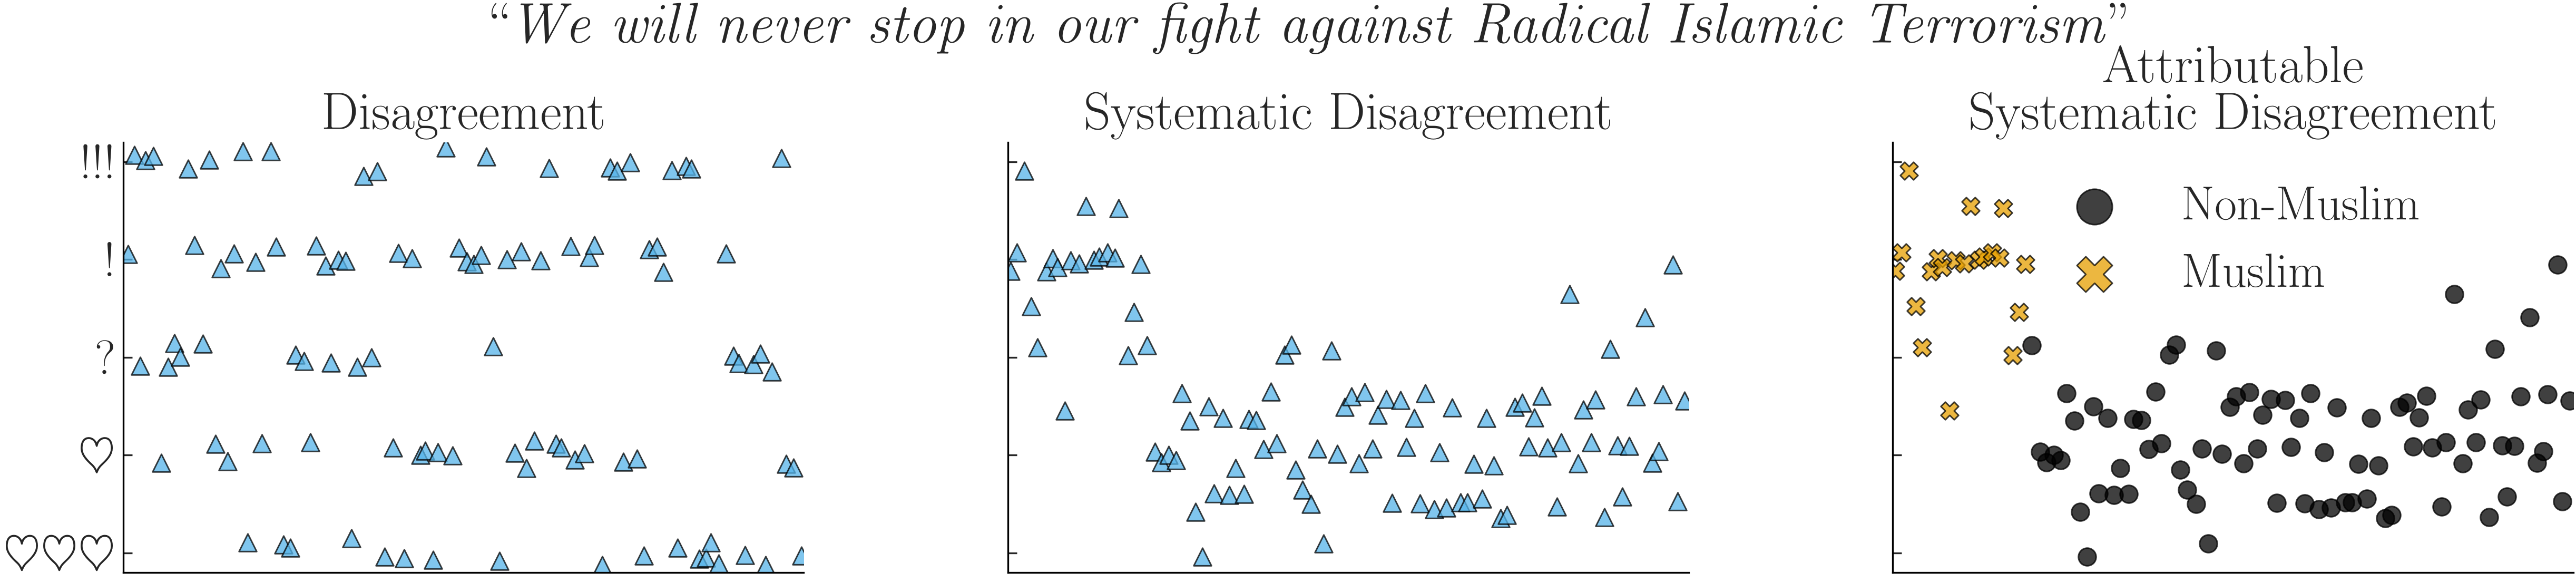
\includegraphics[width=\linewidth]{disagreement_vs_polarization.png}
	\end{frame}
	
	\begin{frame}{Lack of Datasets}
		\resizebox{\textwidth}{!}{%
			\begin{tabular}{lrrrlll}
				\toprule
				\textbf{Dataset} & \textbf{\#Items} & \textbf{\#Ann / Item} & \textbf{PCs} & \textbf{Text Source} & \textbf{Task} & \textbf{Guidelines}\\
				\midrule
				Kumar
				& 1000 & 5   & 10 & Twitter, Reddit, 4chan & Toxicity & Yes \\
				
				Sap
				& 585       & 5--6   & 3  & Twitter & Hate Speech& No  \\
				
				DICES-350
				& 350   & 123    & 4  & LLM responses & Hate Speech & No  \\
				
				DICES-990
				& 990  & 70--76 & 4 &  LLM responses & Hate Speech& No \\
				
				POPQUORN
				& 1500 &7--9 & 5 & Reddit & Hate Speech & Yes \\
				\bottomrule
			\end{tabular}
		}
	\end{frame}
	
	\begin{frame}{Research Questions}
		\begin{enumerate}
			\item How can we \alert{Quantitatively} Attribute Systematic Disagreement to Annotator Groups?
			\item Which \alert{Systematic Disagreement} Patterns are \alert{Shared} Between Human and LLM Annotators?
		\end{enumerate}
	\end{frame}
	
	
	\section{Why Do Current Methods Fail?}
		
	\begin{frame}{On Synthetic Data}
		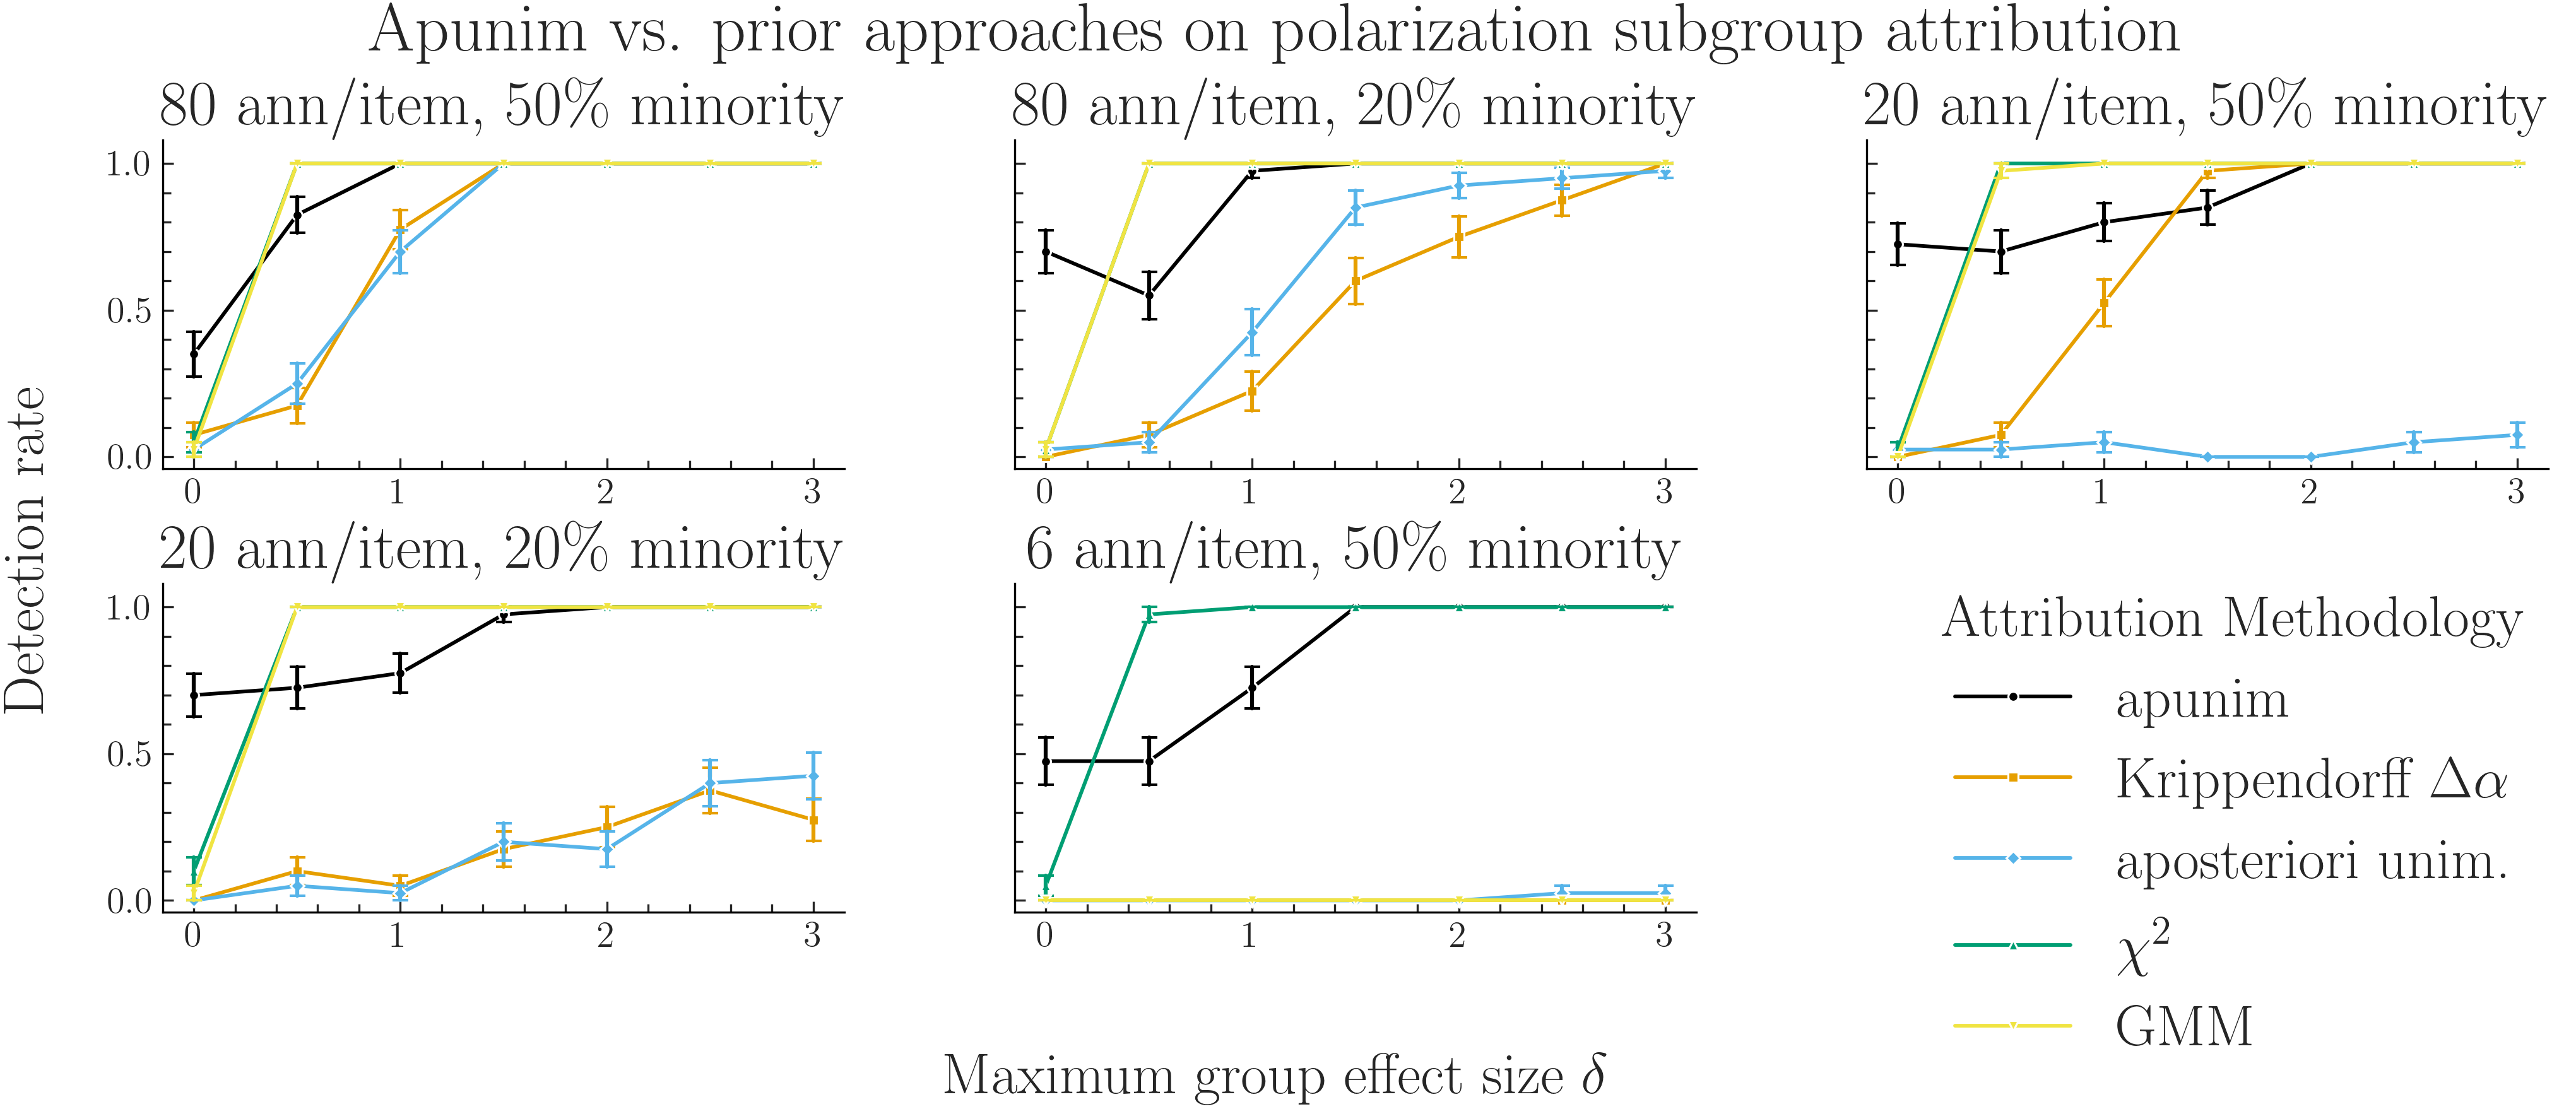
\includegraphics[width=\linewidth]{metric_comparison_simple.png}
	\end{frame}
	
	\begin{frame}{On Real-Life Data}
		\resizebox{\textwidth}{!}{%
			\begin{tabular}{l*{27}{c}}
				\toprule
				& \multicolumn{4}{c}{DICES-350} & \multicolumn{4}{c}{DICES-990} & \multicolumn{3}{c}{Sap et al. 2022} & \multicolumn{11}{c}{Kumar et al. 2021} & \multicolumn{5}{c}{POPQUORN} \\
				\cmidrule(lr){2-5} \cmidrule(lr){6-9} \cmidrule(lr){10-12} \cmidrule(lr){13-23} \cmidrule(lr){24-28}
				\rotatebox{90}{\textbf{Method}} 
				& \rotatebox{90}{Age} & \rotatebox{90}{Education} & \rotatebox{90}{Gender} & \rotatebox{90}{Race}
				& \rotatebox{90}{Age} & \rotatebox{90}{Education} & \rotatebox{90}{Gender} & \rotatebox{90}{Race}
				& \rotatebox{90}{Age} & \rotatebox{90}{Ethnicity} & \rotatebox{90}{Gender}
				& \rotatebox{90}{Age} & \rotatebox{90}{Education} & \rotatebox{90}{Ethnicity} & \rotatebox{90}{Gender/Trans} & \rotatebox{90}{Targeted} & \rotatebox{90}{Parent} & \rotatebox{90}{Politics} & \rotatebox{90}{Religion} & \rotatebox{90}{Tox.Seen/Problem} & \rotatebox{90}{Sex. Orient.} & \rotatebox{90}{Tech Impact}
				& \rotatebox{90}{Age} & \rotatebox{90}{Education} & \rotatebox{90}{Gender} & \rotatebox{90}{Occupation} & \rotatebox{90}{Race} \\
				\midrule
				am
				& \signo & \sigyes & \signo & \sigyes
				& \sigyes & \sigyes & \sigyes & \sigyes
				& \signo & \signo & \sigyes
				& \signo & \signo & \signo & \signo & \signo & \signo & \signo & \signo & \signo & \signo & \signo
				& \signo & \sigyes & \signo & \signo & \sigyes \\
				$\Delta\alpha$
				& \signo & \signo & \sigyes & \sigyes
				& \signo & \sigyes & \sigyes & \signo
				& \signo & \signo & \sigyes
				& \signo & \signo & \signo & \signo & \signo & \signo & \signo & \signo & \signo & \signo & \signo
				& \signo & \signo & \signo & \signo & \signo \\
				AU
				& \signo & \signo & \signo & \signo
				& \signo & \signo & \signo & \signo
				& \signo & \signo & \signo
				& \signo & \signo & \signo & \signo & \signo & \signo & \signo & \signo & \signo & \signo & \signo
				& \signo & \signo & \signo & \signo & \signo \\
				$\chi^2$
				& \sigyes & \sigyes & \sigyes & \sigyes
				& \sigyes & \sigyes & \sigyes & \sigyes
				& \sigyes & \sigyes & \sigyes
				& \sigyes & \sigyes & \sigyes & \sigyes & \sigyes & \sigyes & \sigyes & \sigyes & \sigyes & \sigyes & \sigyes
				& \sigyes & \sigyes & \sigyes & \sigyes & \sigyes \\
				\bottomrule
			\end{tabular}
		}
	\end{frame}
	
	\begin{frame}{Why? Aggregation}
		\begin{figure}[ht]
			\centering
			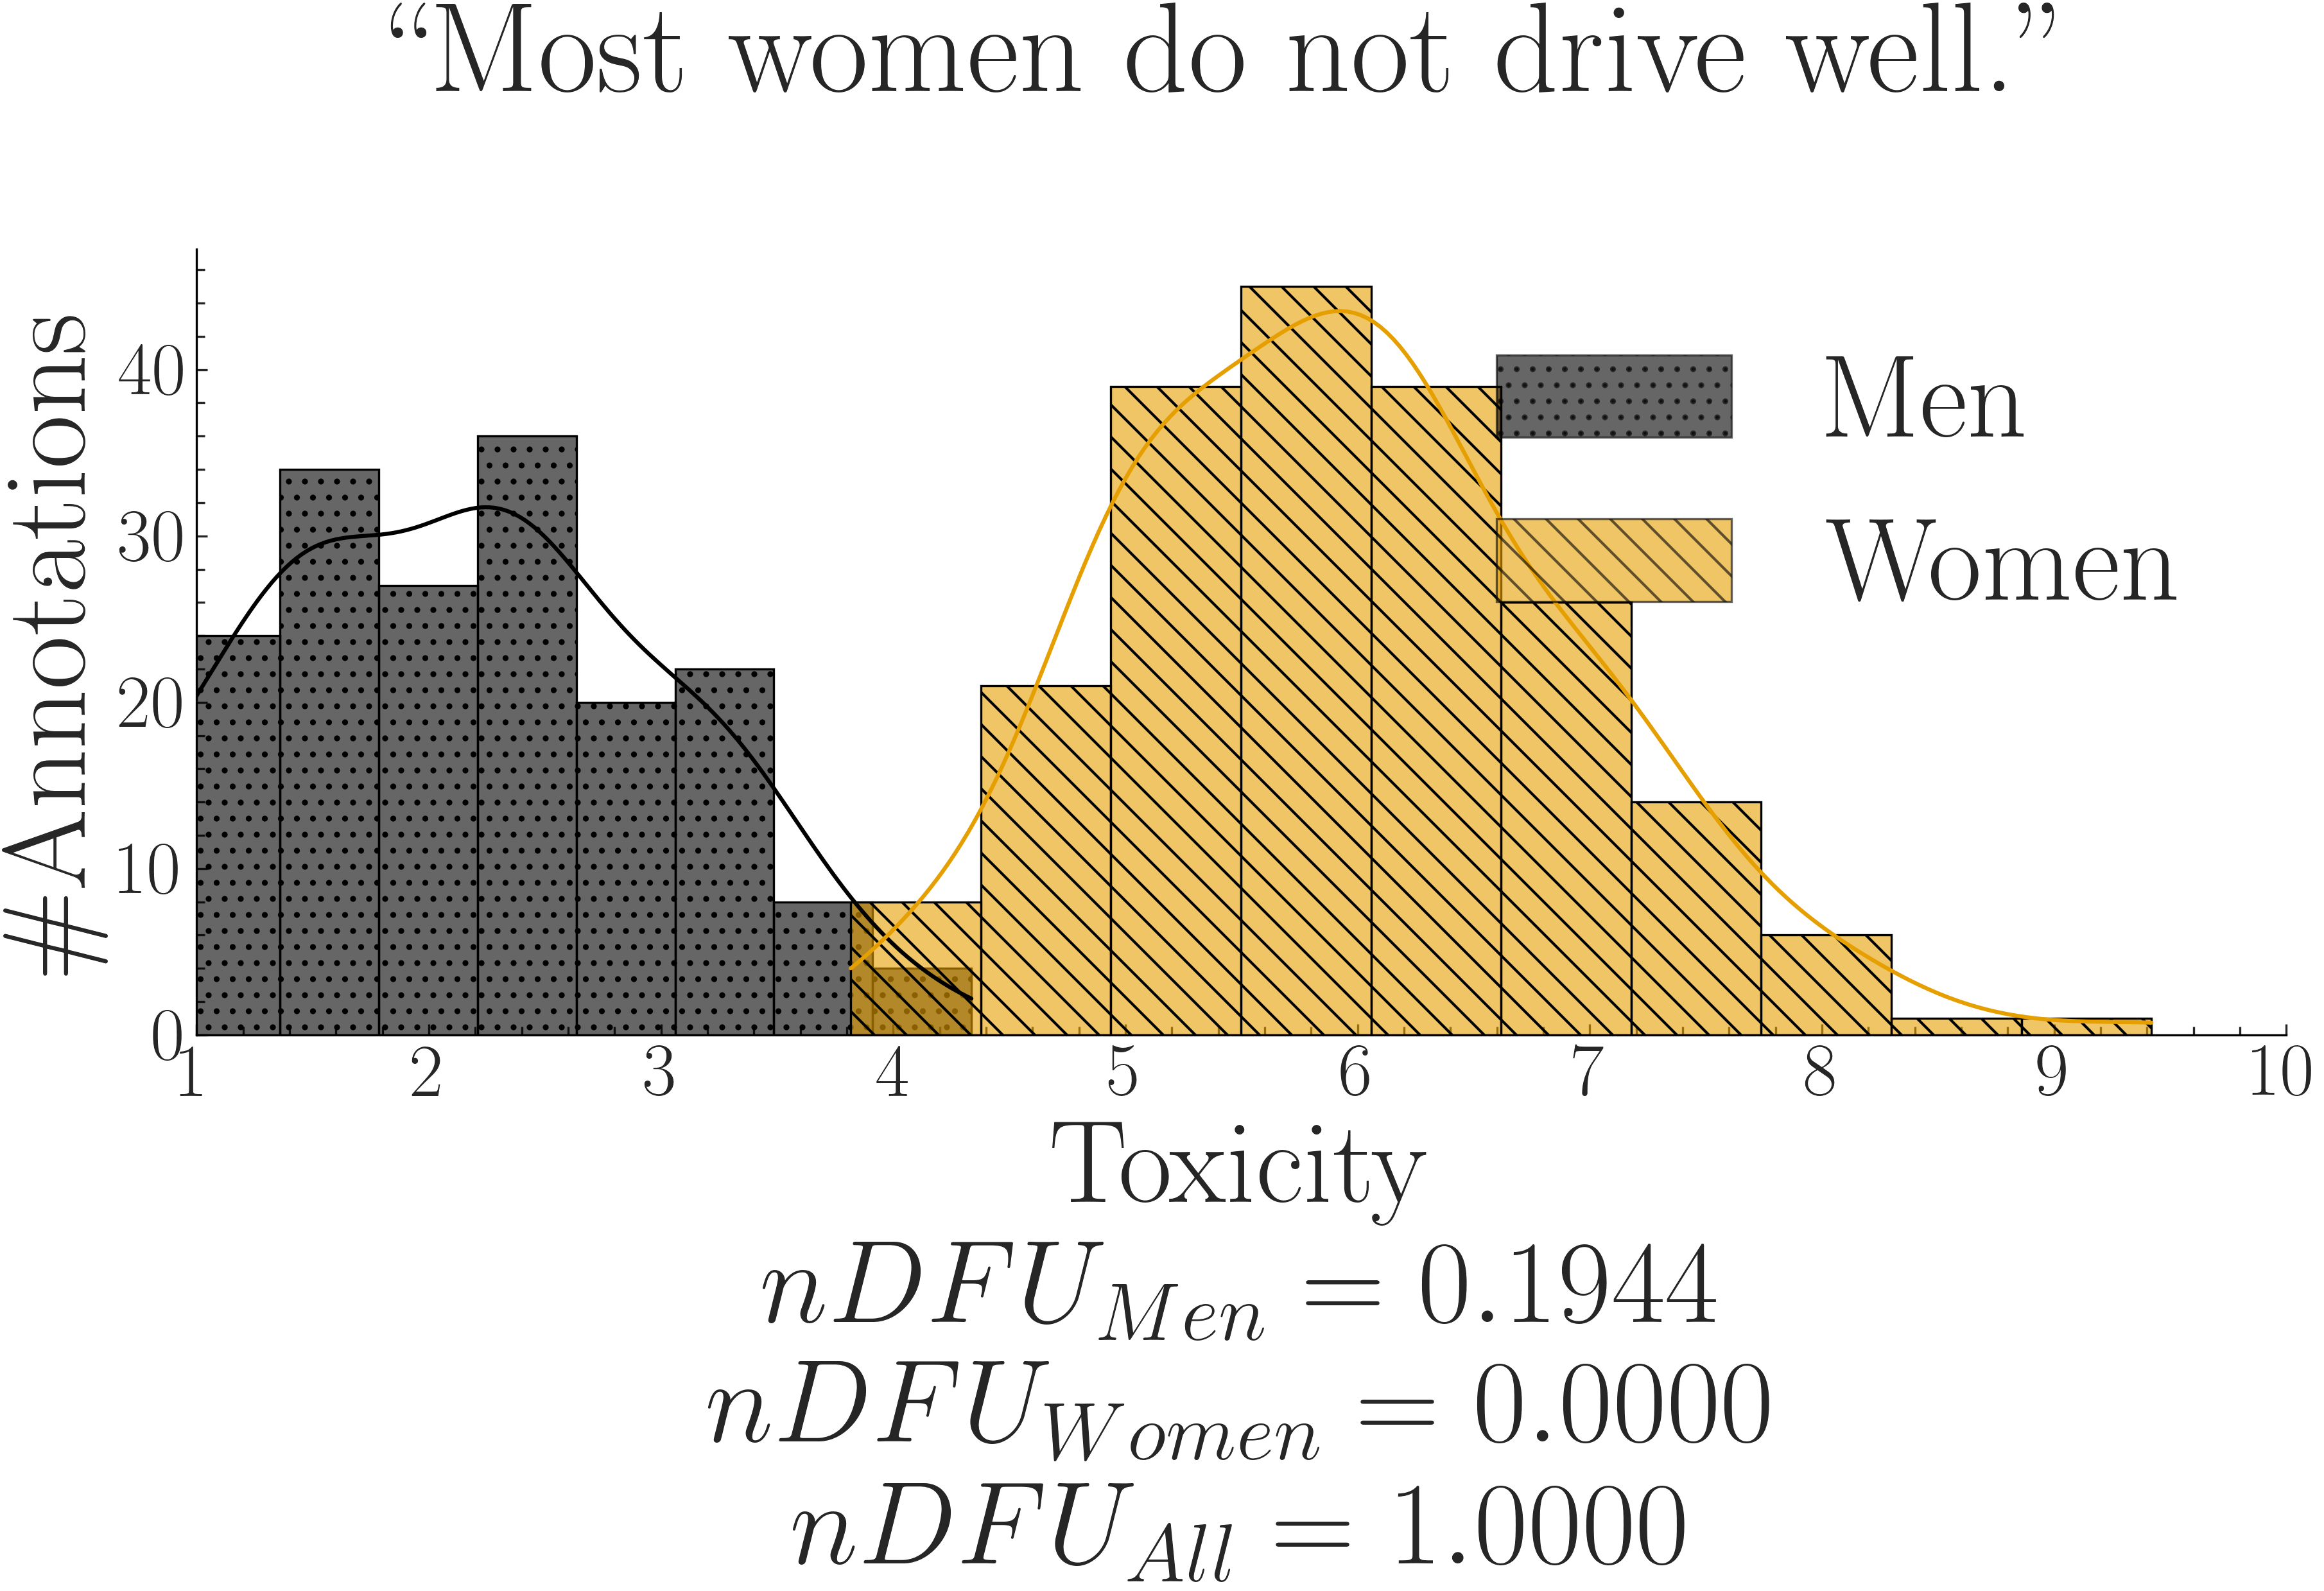
\includegraphics[width=0.4\linewidth]{ndfu_comment1.png}
			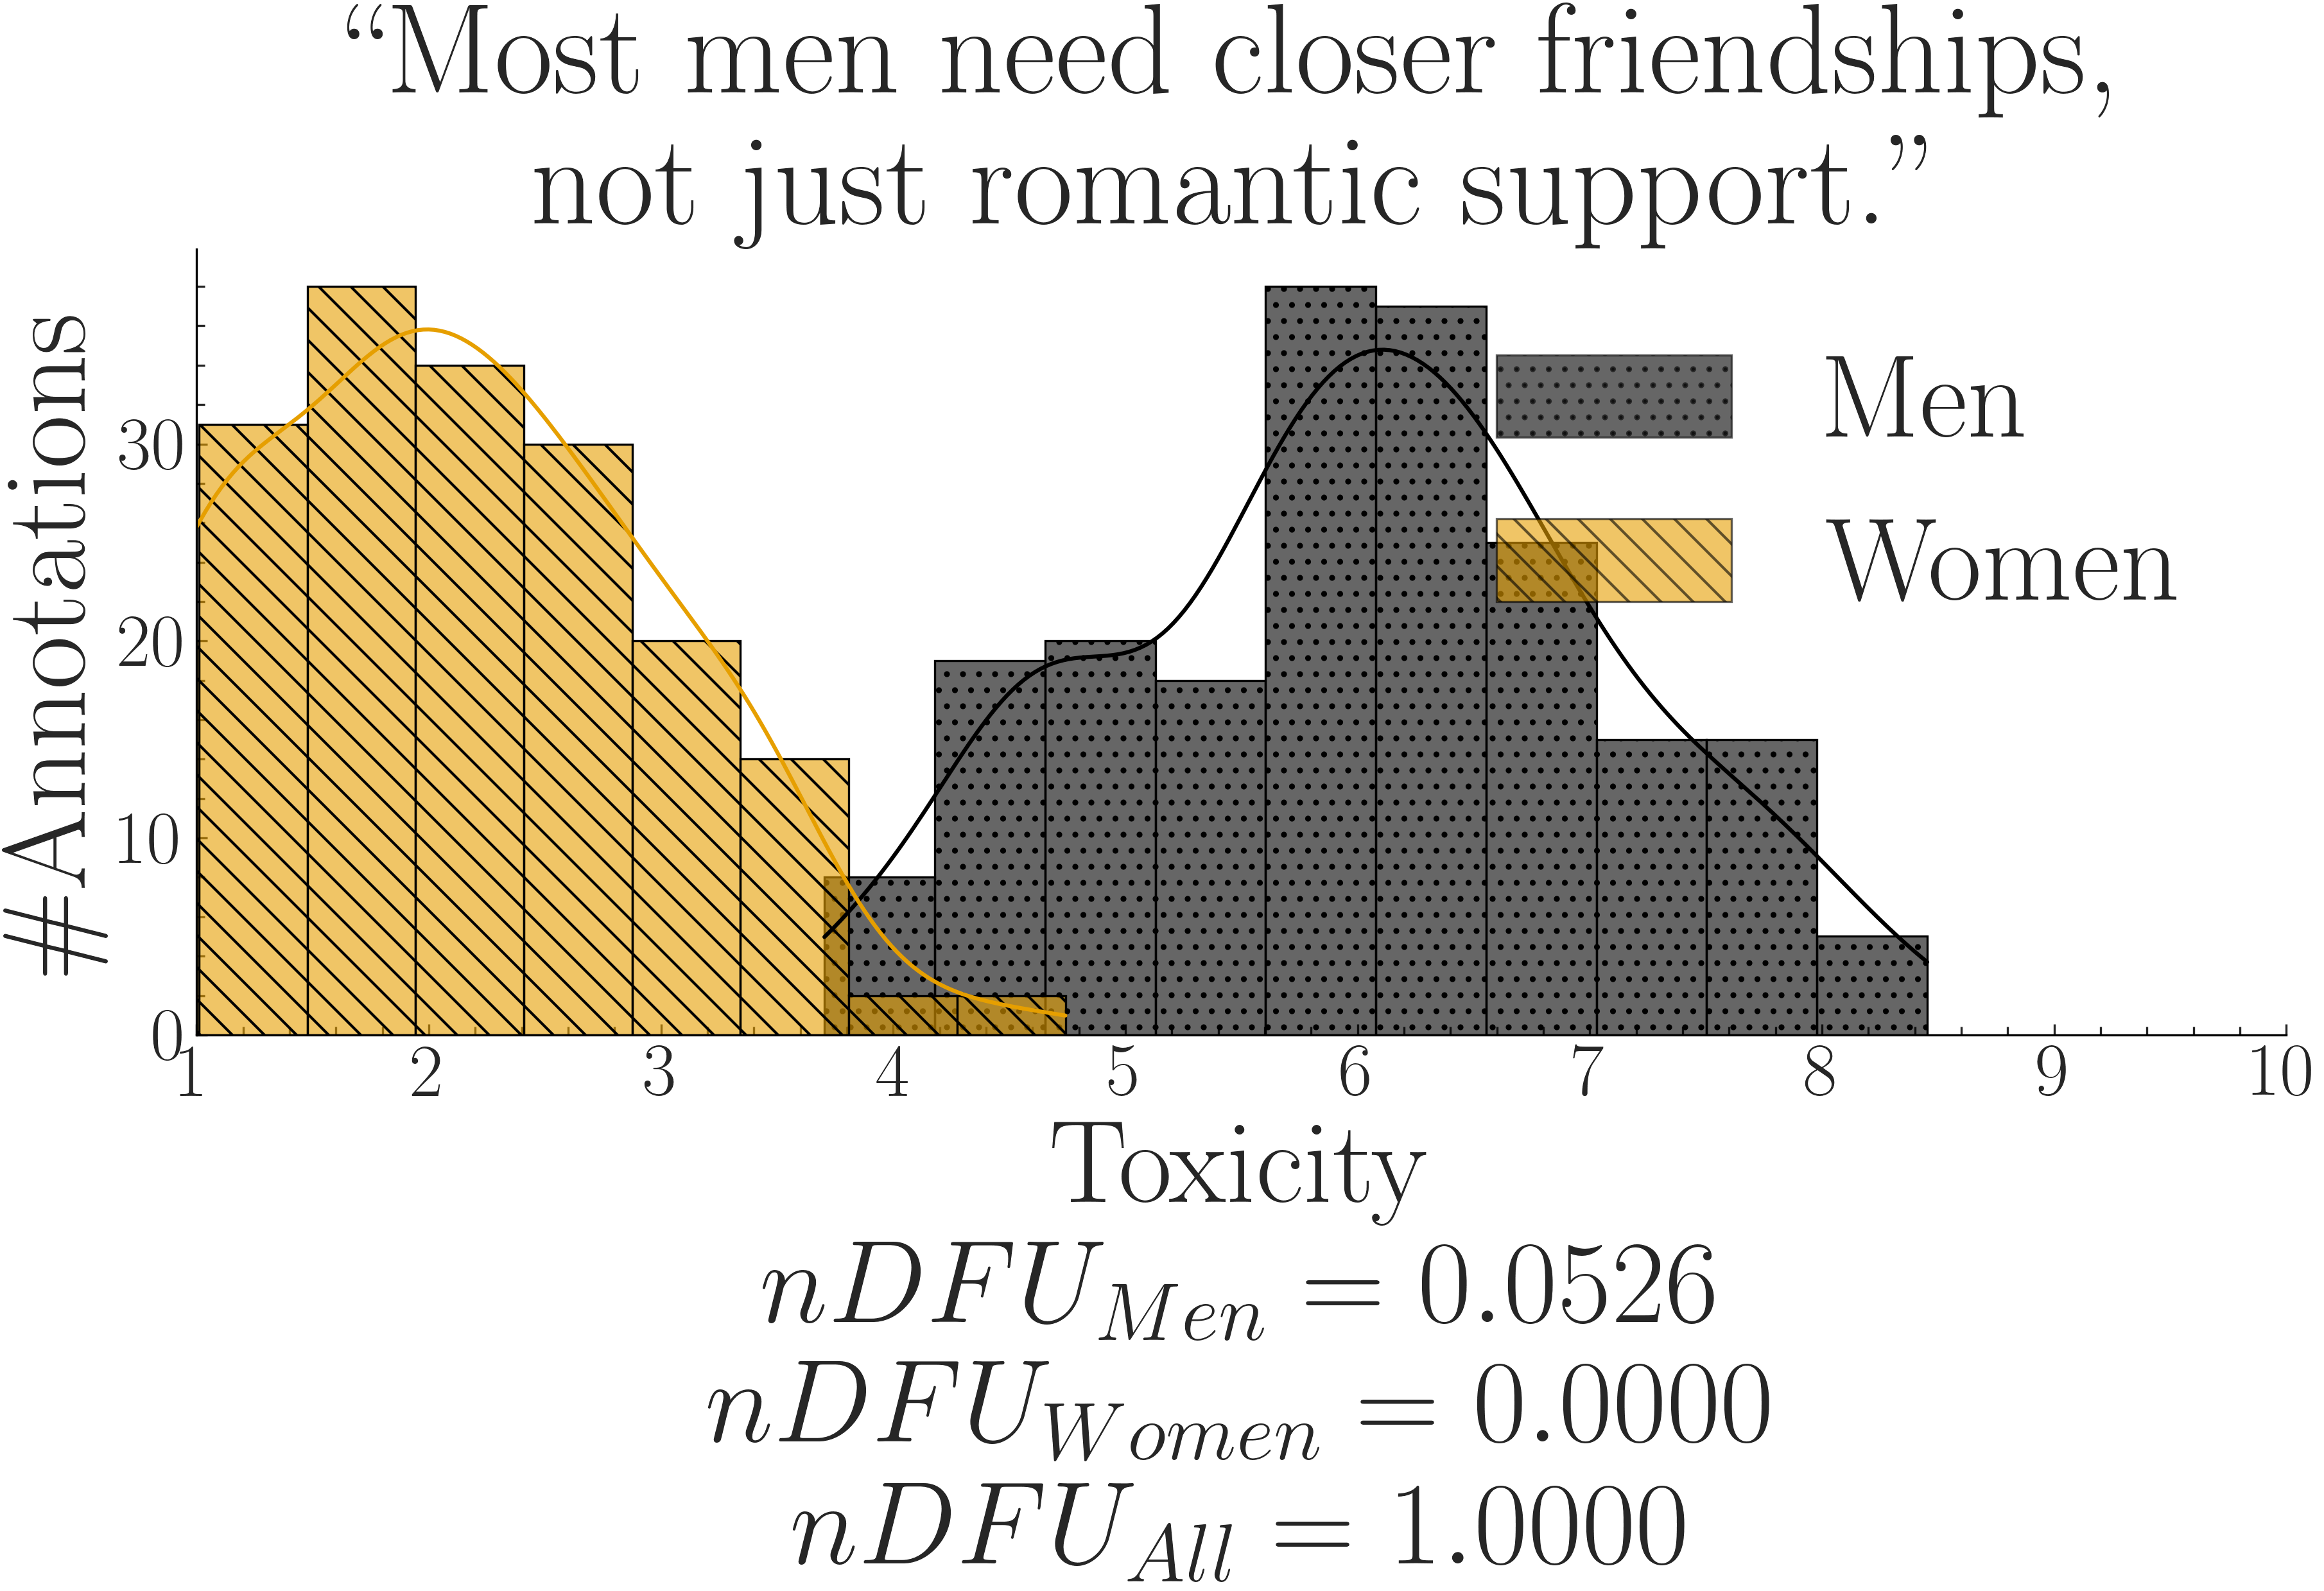
\includegraphics[width=0.4\linewidth]{ndfu_comment2.png}
			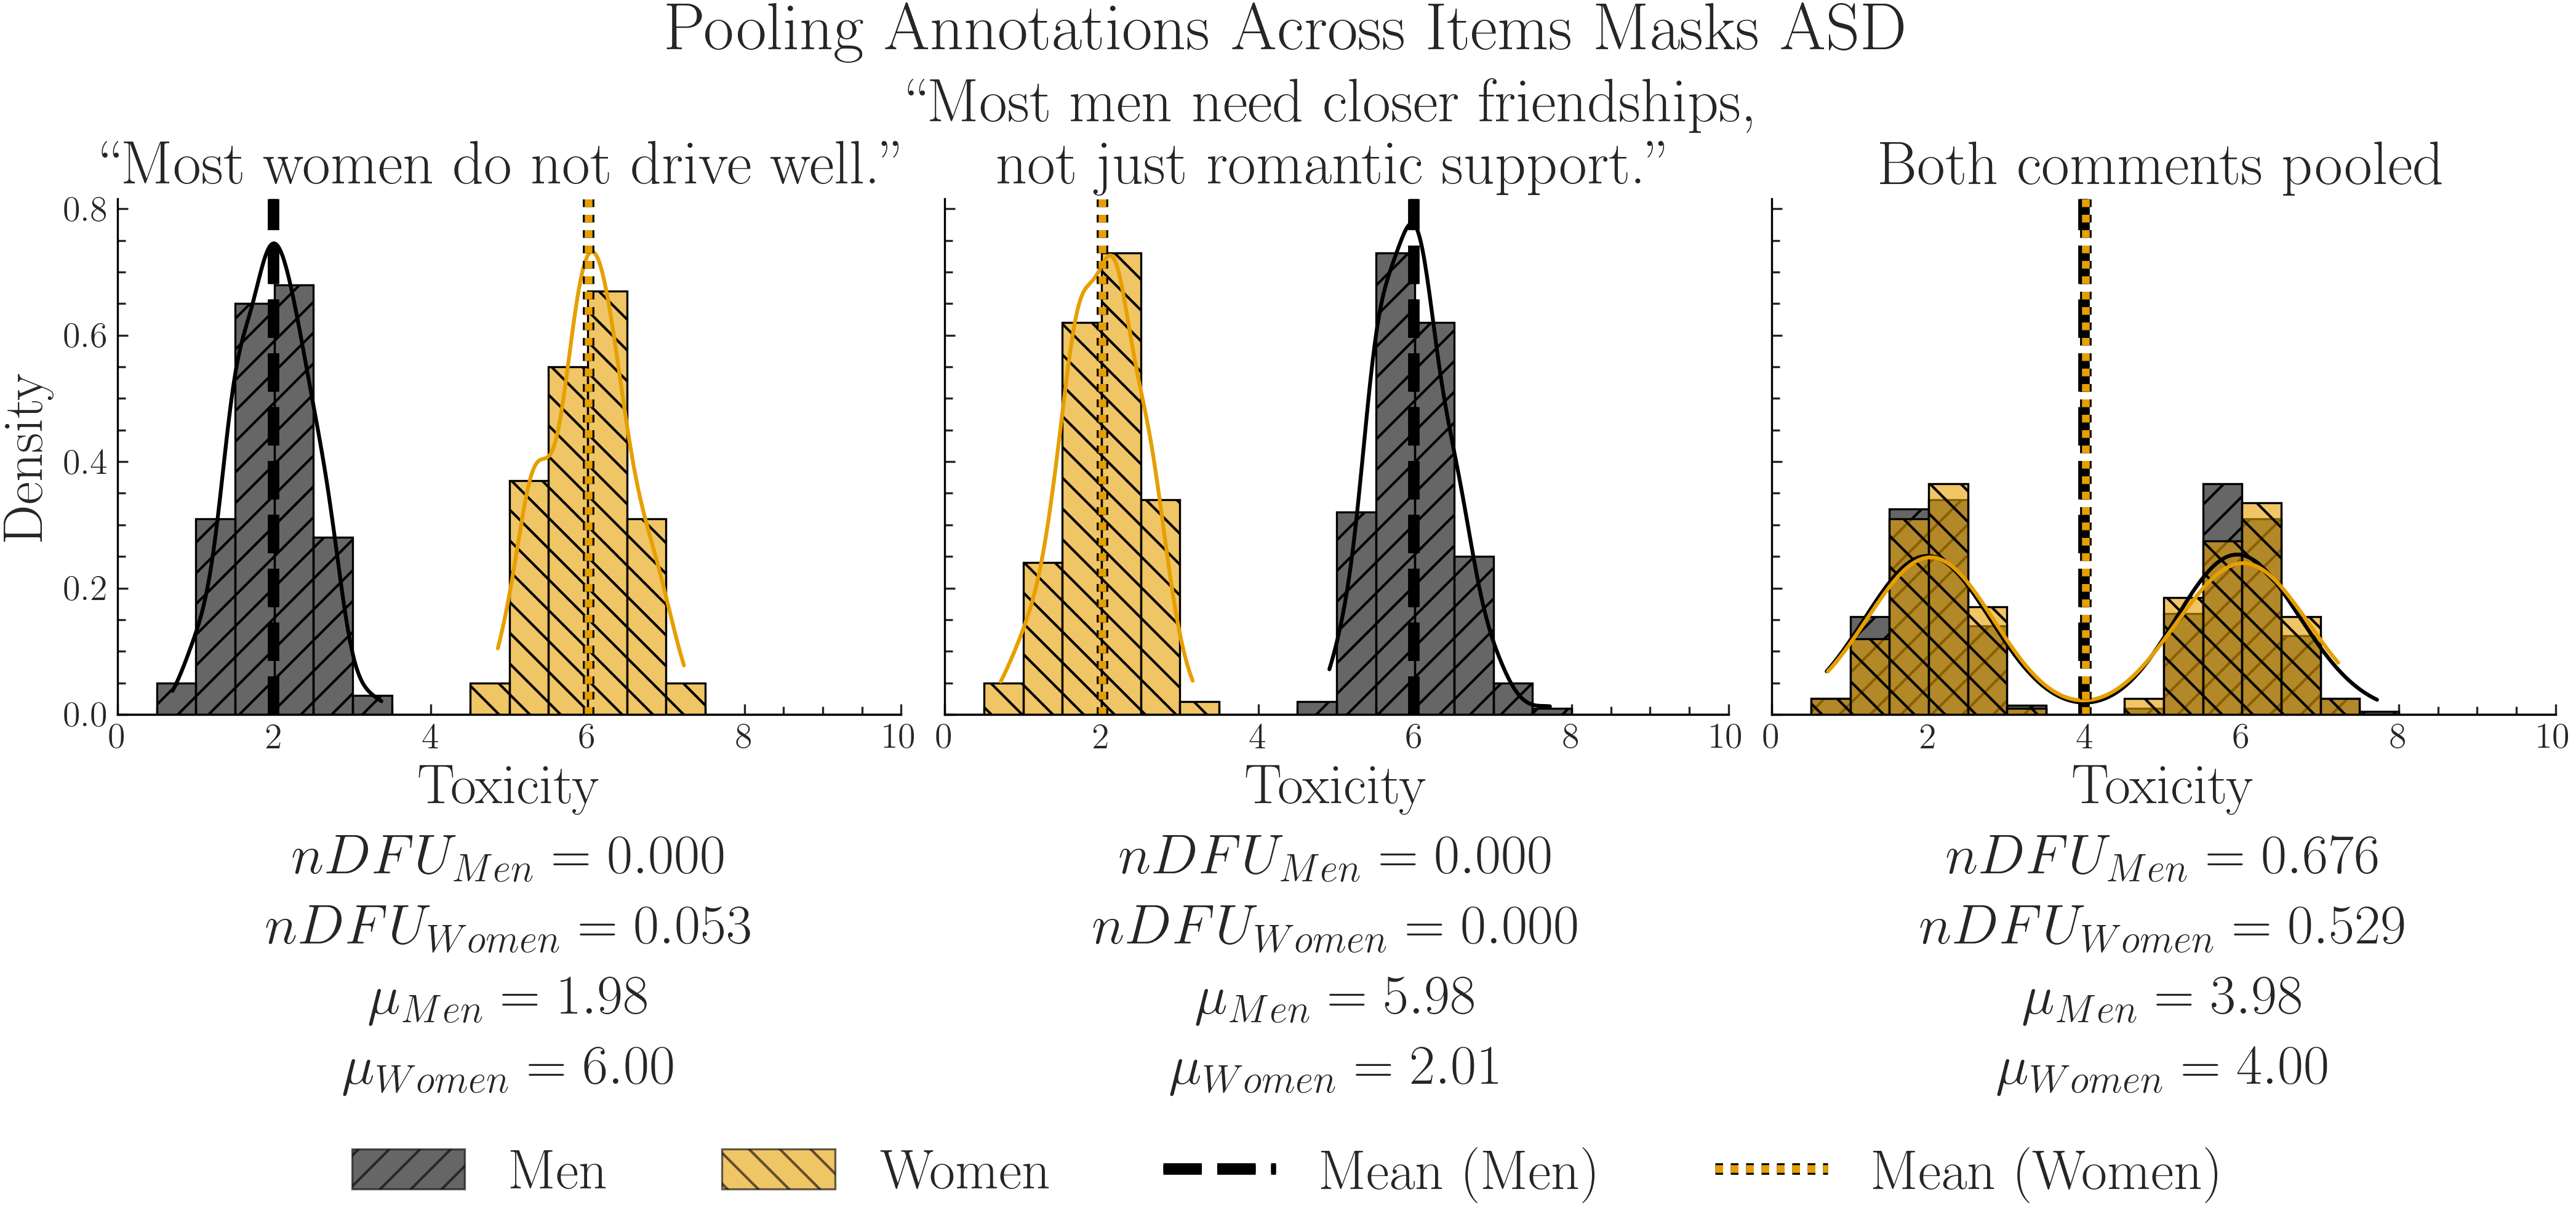
\includegraphics[width=0.4\linewidth]{ndfu_discussion.png}
		\end{figure}
	\end{frame}
	
	\begin{frame}{Why? Unattributable Polarization}
		\begin{columns}
			\begin{column}{0.5\linewidth}
				\resizebox{\columnwidth}{!}{%
					$\begin{aligned}
						\mathrm{Pol}_{inh}(c) &= \min_{S \in G_c} \left\{ \mathrm{nDFU}(S) \right\} \\[1em]
						\mathrm{Pol}_{inh}^{MC}(c) &= \min_{j=1}^{k} \left\{ \mathrm{nDFU}(S_j) \right\}
					\end{aligned}$%
				}
			\end{column}
			\begin{column}{0.5\linewidth}
					\begin{figure}[t]
					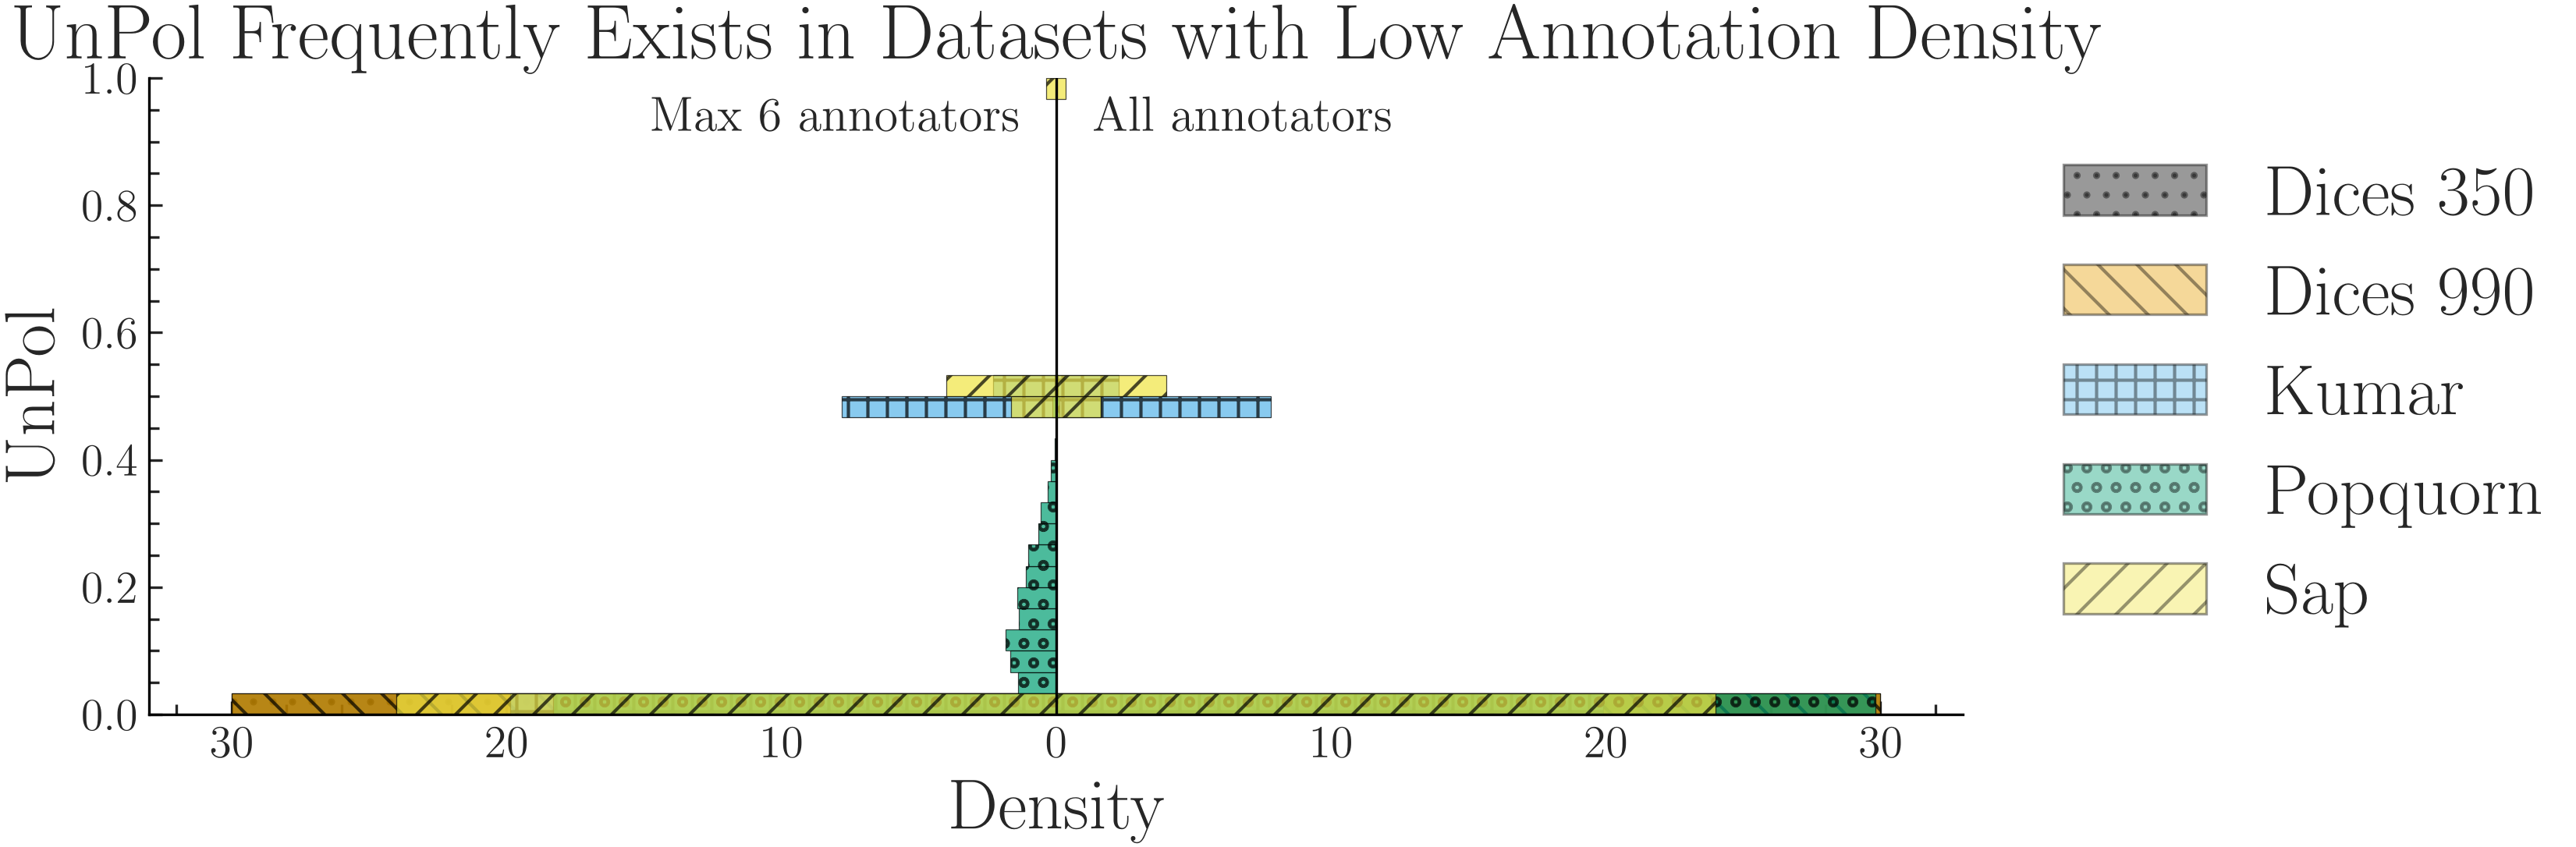
\includegraphics[width=\columnwidth]{apriori.png}
				\end{figure}
			\end{column}
		\end{columns}
	\end{frame}
	
	
	\section{Comparing Human and LLM Polarization}
	
	\begin{frame}{Quantifying Attribution to Annotator Groups}
		\resizebox{\columnwidth}{!}{%
			$apunim(D, g) = \frac{\mathbb{E}_{c \in D} \left[ \mathrm{Pol}_{apr}(c) \right] - \mathbb{E}_{c \in D} \left[ Pol_g(c)\right] }{1 - \mathbb{E}_{c \in D} \left[ \mathrm{Pol}_{apr}(c) \right]}$
		}
	\end{frame}
	
	\begin{frame}{How Are Humans Polarized?}
			\begin{columns}
				\begin{column}{0.45\linewidth}
						\resizebox{\columnwidth}{!}{%
							\begin{tabular}{l r r}
							\toprule
							\textbf{Group} & \textbf{Apunim} & \textbf{Support} \\
							\midrule
							\multicolumn{3}{c}{\textbf{DICES-990}} \\
							\midrule
							\rowcolor{gray!15}
							Ethnicity=AfricanAm & 0.099 & 5148 \\
							\rowcolor{gray!15}
							Ethnicity=Latino & -0.063 & 5877 \\
							\rowcolor{gray!15}
							Ethnicity=Other & 0.034 & 21669 \\
							\rowcolor{gray!15}
							Ethnicity=White & -0.065 & 10166 \\
							\rowcolor{gray!15}
							Gender=Man & 0.036 & 28817 \\
							\rowcolor{gray!15}
							Gender=Woman & -0.027 & 29990 \\
							Age=GenZ & 0.047 & 12214 \\
							Age=Millennial & -0.007 & 34433 \\
							Age=GenX+ & -0.028 & 12699 \\
							Education=College & 0.006 & 52727 \\
							Education=High school & -0.050 & 6619 \\
							\bottomrule
						\end{tabular}
					}
				\end{column}
				\begin{column}{0.45\linewidth}
					\resizebox{\columnwidth}{!}{%
						\begin{tabular}{l r r}
							\toprule
							\textbf{Group} & \textbf{Apunim} & \textbf{Support} \\
							\midrule
							\multicolumn{3}{c}{\textbf{DICES-350}} \\
							\midrule
							\rowcolor{gray!15}
							Ethnicity=AfricanAm & -0.037 & 7627 \\
							\rowcolor{gray!15}
							Ethnicity=Asian & 0.045 & 6838 \\
							Education=Other & -0.023 & 1841 \\
							\midrule
							\multicolumn{3}{c}{\textbf{Sap}} \\
							\midrule
							\rowcolor{gray!15}
							Gender=Man & 0.0907 & 1439 \\
							\rowcolor{gray!15}
							Gender=Woman & -0.2442 & 877 \\
							\midrule
							\multicolumn{3}{c}{\textbf{POPQUORN}} \\
							\midrule
							\rowcolor{gray!15}
							Gender=Man & 0.0081 & 2720 \\
							\rowcolor{gray!15}
							Race=Black & -0.1572 & 222 \\
							Education=College & 0.0496& 2388 \\
							Education=Graduate & -0.0808 & 468 \\
							\bottomrule
						\end{tabular}
					}
					\end{column}
		\end{columns}
	\end{frame}
	
	\begin{frame}{How Are LLMs Polarized? Unimodality}
		\resizebox{\linewidth}{!}{
			\begin{tabular}{lrrrrrrrr}
				\toprule
				& \multicolumn{2}{c}{Sap et al. 2022} & \multicolumn{2}{c}{Kumar et al. 2021} & \multicolumn{2}{c}{POPQUORN} & \multicolumn{2}{c}{All} \\
				& n & Mean (SE) & n & Mean (SE) & n & Mean (SE) & n & Mean (SE) \\
				Model &  &  &  &  &  &  &  &  \\
				\midrule
				Human & 585 & 0.38 (0.01) & 1000 & 0.42 (0.01) & 1500 & 0.31 (0.01) & 3085 & 0.36 (0.00) \\
				olmo32b & 585 & 0.24 (0.01) & 1000 & 0.51 (0.01) & 1500 & 0.50 (0.01) & 3085 & 0.45 (0.01) \\
				qwen32b & 585 & 0.18 (0.01) & 1000 & 0.19 (0.01) & 1499 & 0.20 (0.01) & 3084 & 0.19 (0.00) \\
				mistral7b & 585 & 0.21 (0.01) & --- & --- & 1500 & 0.40 (0.01) & 2085 & 0.34 (0.01) \\
				mistral24b & 585 & 0.25 (0.01) & --- & --- & 1500 & 0.23 (0.01) & 2085 & 0.24 (0.01) \\
				gemma7b & 585 & 0.19 (0.01) & --- & --- & 1500 & 0.12 (0.01) & 2085 & 0.14 (0.01) \\
				gemma31b & 585 & 0.04 (0.01) & --- & --- & 1500 & 0.05 (0.00) & 2085 & 0.05 (0.00) \\
				\bottomrule
			\end{tabular}
		}
	\end{frame}
	
	\begin{frame}{How Are LLMs Polarized? Unattributable}
		\begin{center}
				\resizebox{0.5\linewidth}{!}{
				\begin{tabular}{llrrrrr}
					\toprule
					&  & n & Stereotype & Persona & Single & Direct \\
					Model & Dataset &  &  &  &  &  \\
					\midrule
					\multirow[t]{4}{*}{olmo32b} & All & 3085 & -0.09 & -0.02 & 0.01 & -0.15 \\
					& Sap et al. 2022 & 585 & 0.09 & 0.06 & 0.22 & 0.04 \\
					& Kumar et al. 2021 & 1000 & 0.14 & -0.13 & -0.29 & -0.31 \\
					& POPQUORN & 1500 & -0.50 & -0.00 & 0.10 & -0.19 \\
					\cline{1-7}
					\multirow[t]{4}{*}{qwen32b} & All & 3084 & 0.25 & 0.22 & 0.22 & 0.19 \\
					& Sap et al. 2022 & 585 & 0.32 & 0.13 & -0.09 & 0.09 \\
					& Kumar et al. 2021 & 1000 & 0.17 & 0.21 & 0.51 & 0.31 \\
					& POPQUORN & 1499 & 0.26 & 0.30 & 0.24 & 0.17 \\
					\cline{1-7}
					\multirow[t]{3}{*}{mistral7b} & All & 2085 & 0.16 & 0.06 & 0.21 & 0.10 \\
					& Sap et al. 2022 & 585 & 0.21 & 0.10 & 0.08 & 0.57 \\
					& POPQUORN & 1500 & 0.12 & 0.02 & 0.33 & -0.36 \\
					\cline{1-7}
					\multirow[t]{3}{*}{mistral24b} & All & 2085 & 0.60 & 0.12 & -0.53 & 0.31 \\
					& Sap et al. 2022 & 585 & 0.64 & 0.04 & -0.76 & 0.27 \\
					& POPQUORN & 1500 & 0.55 & 0.20 & -0.30 & 0.35 \\
					\cline{1-7}
					\multirow[t]{3}{*}{gemma7b} & All & 2085 & 0.26 & 0.51 & 0.78 & 0.39 \\
					& Sap et al. 2022 & 585 & 0.18 & 0.48 & 0.57 & 0.15 \\
					& POPQUORN & 1500 & 0.34 & 0.54 & 0.99 & 0.63 \\
					\cline{1-7}
					\multirow[t]{3}{*}{gemma31b} & All & 2085 & 0.42 & 0.31 & 0.00 & 0.63 \\
					& Sap et al. 2022 & 585 & 0.36 & 0.21 & 0.06 & 1.03 \\
					& POPQUORN & 1500 & 0.47 & 0.40 & -0.06 & 0.23 \\
					\cline{1-7}
					\bottomrule
				\end{tabular}
			}
		\end{center}
	\end{frame}
	
	\begin{frame}{How Are LLMs Polarized? Group Attribution}
		\resizebox{\linewidth}{!}{
			\begin{tabular}{llcccccc}
				\toprule
				&  & olmo32b & qwen32b & mistral7b & mistral24b & gemma7b & gemma31b \\
				\midrule
				Dataset & PC &  &  &  &  &  &  \\
				\midrule
				\multirow[t]{3}{*}{Sap et al. 2022} & Age & \makebox[1.2em][c]{\signo}\makebox[1.2em][c]{\signo}\makebox[1.2em][c]{\signo}\makebox[1.2em][c]{\sigyes}\makebox[1.2em][c]{\signo} & \makebox[1.2em][c]{\signo}\makebox[1.2em][c]{\signo}\makebox[1.2em][c]{\signo}\makebox[1.2em][c]{\signo}\makebox[1.2em][c]{\signo} & \makebox[1.2em][c]{\signo}\makebox[1.2em][c]{\signo}\makebox[1.2em][c]{\signo}\makebox[1.2em][c]{\sigyes}\makebox[1.2em][c]{\signo} & \makebox[1.2em][c]{\signo}\makebox[1.2em][c]{\signo}\makebox[1.2em][c]{\signo}\makebox[1.2em][c]{\signo}\makebox[1.2em][c]{\signo} & \makebox[1.2em][c]{\sigyes}\makebox[1.2em][c]{\sigyes}\makebox[1.2em][c]{\signo}\makebox[1.2em][c]{\sigyes}\makebox[1.2em][c]{\signo} & \makebox[1.2em][c]{\signo}\makebox[1.2em][c]{\signo}\makebox[1.2em][c]{\signo}\makebox[1.2em][c]{\signo}\makebox[1.2em][c]{\signo} \\
				& Ethnicity & \makebox[1.2em][c]{\sigyes}\makebox[1.2em][c]{\sigyes}\makebox[1.2em][c]{\signo}\makebox[1.2em][c]{\sigyes}\makebox[1.2em][c]{\signo} & \makebox[1.2em][c]{\signo}\makebox[1.2em][c]{\signo}\makebox[1.2em][c]{\signo}\makebox[1.2em][c]{\signo}\makebox[1.2em][c]{\signo} & \makebox[1.2em][c]{\signo}\makebox[1.2em][c]{\signo}\makebox[1.2em][c]{\signo}\makebox[1.2em][c]{\signo}\makebox[1.2em][c]{\signo} & \makebox[1.2em][c]{\signo}\makebox[1.2em][c]{\signo}\makebox[1.2em][c]{\sigyes}\makebox[1.2em][c]{\signo}\makebox[1.2em][c]{\signo} & \makebox[1.2em][c]{\signo}\makebox[1.2em][c]{\signo}\makebox[1.2em][c]{\signo}\makebox[1.2em][c]{\signo}\makebox[1.2em][c]{\signo} & \makebox[1.2em][c]{\signo}\makebox[1.2em][c]{\signo}\makebox[1.2em][c]{\signo}\makebox[1.2em][c]{\signo}\makebox[1.2em][c]{\signo} \\
				& Gender & \makebox[1.2em][c]{\signo}\makebox[1.2em][c]{\signo}\makebox[1.2em][c]{\signo}\makebox[1.2em][c]{\signo}\makebox[1.2em][c]{\signo} & \makebox[1.2em][c]{\signo}\makebox[1.2em][c]{\sigyes}\makebox[1.2em][c]{\signo}\makebox[1.2em][c]{\signo}\makebox[1.2em][c]{$\pm$} & \makebox[1.2em][c]{\signo}\makebox[1.2em][c]{\sigyes}\makebox[1.2em][c]{\sigyes}\makebox[1.2em][c]{\signo}\makebox[1.2em][c]{\signo} & \makebox[1.2em][c]{$\pm$}\makebox[1.2em][c]{\sigyes}\makebox[1.2em][c]{\sigyes}\makebox[1.2em][c]{\sigyes}\makebox[1.2em][c]{$\pm$} & \makebox[1.2em][c]{\signo}\makebox[1.2em][c]{\signo}\makebox[1.2em][c]{$\pm$}\makebox[1.2em][c]{\signo}\makebox[1.2em][c]{$\pm$} & \makebox[1.2em][c]{\signo}\makebox[1.2em][c]{\signo}\makebox[1.2em][c]{\signo}\makebox[1.2em][c]{\signo}\makebox[1.2em][c]{\sigyes} \\
				\cline{1-8}
				\multirow[t]{5}{*}{POPQUORN} & Age & \makebox[1.2em][c]{\signo}\makebox[1.2em][c]{\signo}\makebox[1.2em][c]{\sigyes}\makebox[1.2em][c]{\signo}\makebox[1.2em][c]{\signo} & \makebox[1.2em][c]{\signo}\makebox[1.2em][c]{\signo}\makebox[1.2em][c]{\signo}\makebox[1.2em][c]{\signo}\makebox[1.2em][c]{\signo} & \makebox[1.2em][c]{\signo}\makebox[1.2em][c]{\signo}\makebox[1.2em][c]{\signo}\makebox[1.2em][c]{\signo}\makebox[1.2em][c]{\signo} & \makebox[1.2em][c]{\signo}\makebox[1.2em][c]{\signo}\makebox[1.2em][c]{\signo}\makebox[1.2em][c]{\signo}\makebox[1.2em][c]{\signo} & \makebox[1.2em][c]{\signo}\makebox[1.2em][c]{\signo}\makebox[1.2em][c]{\signo}\makebox[1.2em][c]{\signo}\makebox[1.2em][c]{\signo} & \makebox[1.2em][c]{\signo}\makebox[1.2em][c]{\signo}\makebox[1.2em][c]{\signo}\makebox[1.2em][c]{\signo}\makebox[1.2em][c]{\sigyes} \\
				& Education & \makebox[1.2em][c]{\sigyes}\makebox[1.2em][c]{\sigyes}\makebox[1.2em][c]{$\pm$}\makebox[1.2em][c]{\sigyes}\makebox[1.2em][c]{\sigyes} & \makebox[1.2em][c]{$\pm$}\makebox[1.2em][c]{$\pm$}\makebox[1.2em][c]{$\pm$}\makebox[1.2em][c]{\sigyes}\makebox[1.2em][c]{$\pm$} & \makebox[1.2em][c]{\sigyes}\makebox[1.2em][c]{\sigyes}\makebox[1.2em][c]{\sigyes}\makebox[1.2em][c]{\sigyes}\makebox[1.2em][c]{\sigyes} & \makebox[1.2em][c]{\sigyes}\makebox[1.2em][c]{\sigyes}\makebox[1.2em][c]{\sigyes}\makebox[1.2em][c]{\sigyes}\makebox[1.2em][c]{\sigyes} & \makebox[1.2em][c]{\signo}\makebox[1.2em][c]{\signo}\makebox[1.2em][c]{\sigyes}\makebox[1.2em][c]{\sigyes}\makebox[1.2em][c]{\sigyes} & \makebox[1.2em][c]{\signo}\makebox[1.2em][c]{$\pm$}\makebox[1.2em][c]{$\pm$}\makebox[1.2em][c]{\signo}\makebox[1.2em][c]{\signo} \\
				& Gender & \makebox[1.2em][c]{\sigyes}\makebox[1.2em][c]{\sigyes}\makebox[1.2em][c]{\sigyes}\makebox[1.2em][c]{\sigyes}\makebox[1.2em][c]{\signo} & \makebox[1.2em][c]{\sigyes}\makebox[1.2em][c]{\signo}\makebox[1.2em][c]{\signo}\makebox[1.2em][c]{\signo}\makebox[1.2em][c]{\signo} & \makebox[1.2em][c]{\signo}\makebox[1.2em][c]{\sigyes}\makebox[1.2em][c]{\signo}\makebox[1.2em][c]{\sigyes}\makebox[1.2em][c]{\signo} & \makebox[1.2em][c]{\signo}\makebox[1.2em][c]{\signo}\makebox[1.2em][c]{\signo}\makebox[1.2em][c]{\signo}\makebox[1.2em][c]{\signo} & \makebox[1.2em][c]{\signo}\makebox[1.2em][c]{\signo}\makebox[1.2em][c]{\signo}\makebox[1.2em][c]{\signo}\makebox[1.2em][c]{\signo} & \makebox[1.2em][c]{\signo}\makebox[1.2em][c]{\signo}\makebox[1.2em][c]{\signo}\makebox[1.2em][c]{\signo}\makebox[1.2em][c]{\signo} \\
				& Occupation & \makebox[1.2em][c]{\signo}\makebox[1.2em][c]{\signo}\makebox[1.2em][c]{\sigyes}\makebox[1.2em][c]{\sigyes}\makebox[1.2em][c]{\sigyes} & \makebox[1.2em][c]{\sigyes}\makebox[1.2em][c]{\sigyes}\makebox[1.2em][c]{\sigyes}\makebox[1.2em][c]{\signo}\makebox[1.2em][c]{\signo} & \makebox[1.2em][c]{$\pm$}\makebox[1.2em][c]{$\pm$}\makebox[1.2em][c]{$\pm$}\makebox[1.2em][c]{\sigyes}\makebox[1.2em][c]{\sigyes} & \makebox[1.2em][c]{\sigyes}\makebox[1.2em][c]{$\pm$}\makebox[1.2em][c]{\sigyes}\makebox[1.2em][c]{\sigyes}\makebox[1.2em][c]{\sigyes} & \makebox[1.2em][c]{\sigyes}\makebox[1.2em][c]{$\pm$}\makebox[1.2em][c]{$\pm$}\makebox[1.2em][c]{\sigyes}\makebox[1.2em][c]{\signo} & \makebox[1.2em][c]{\signo}\makebox[1.2em][c]{\signo}\makebox[1.2em][c]{\sigyes}\makebox[1.2em][c]{\signo}\makebox[1.2em][c]{\signo} \\
				& Race & \makebox[1.2em][c]{\sigyes}\makebox[1.2em][c]{\signo}\makebox[1.2em][c]{\sigyes}\makebox[1.2em][c]{\sigyes}\makebox[1.2em][c]{\sigyes} & \makebox[1.2em][c]{$\pm$}\makebox[1.2em][c]{$\pm$}\makebox[1.2em][c]{$\pm$}\makebox[1.2em][c]{\sigyes}\makebox[1.2em][c]{\sigyes} & \makebox[1.2em][c]{\sigyes}\makebox[1.2em][c]{$\pm$}\makebox[1.2em][c]{$\pm$}\makebox[1.2em][c]{\sigyes}\makebox[1.2em][c]{$\pm$} & \makebox[1.2em][c]{$\pm$}\makebox[1.2em][c]{$\pm$}\makebox[1.2em][c]{\sigyes}\makebox[1.2em][c]{\sigyes}\makebox[1.2em][c]{$\pm$} & \makebox[1.2em][c]{$\pm$}\makebox[1.2em][c]{$\pm$}\makebox[1.2em][c]{\sigyes}\makebox[1.2em][c]{$\pm$}\makebox[1.2em][c]{$\pm$} & \makebox[1.2em][c]{$\pm$}\makebox[1.2em][c]{$\pm$}\makebox[1.2em][c]{$\pm$}\makebox[1.2em][c]{\sigyes}\makebox[1.2em][c]{\sigyes} \\
				\cline{1-8}
			\end{tabular}
		}
	\end{frame}

\end{document}